\section{Movement Recognition}\label{5_3_movementRecognition}
%- Recording of gestures --> Kinectstudio --> Making/Train gestures --> Visual gestures builder
The SLS guides the trainee through predefined exercises for slacklining. In the case of this thesis it is important to know that exercises are defined as \textit{gestures} within the context of the Kinect development. The \textit{Kinect for Windows Human Interface Guidelines} describe the term gesture as follows: "\textit{[...] we use the term gesture broadly to mean any form of movement that can be used as an input or interaction to control or influence an application.}"~\cite{MicrosoftHIG2014-mh}.

\subsection{Heuristics vs. Visual Gesture Builder}
The Kinect SDK provides two approaches for tracking a gesture in an application~\cite{MicrosoftVGB}.
The first one is called heuristic approach, which means to manually track each body joint position of the user in the code.
Conditions can be defined according to the action that should happen e.g. if a joint exceeds a certain threshold or is in a defined range.
Heuristics are mainly used for simple gestures like raising the hand over the head, which is implemented in the SLS as engagement gesture.
For more complex gestures, the developer must have a good understanding about the movement and behaviour of the human body.
Furthermore, environmental factors like an inappropriate mounting of the Kinect could exacerbate managing and maintaining the code.

Usually a common developer has not the appropriate expertise of the human body behaviour or it would take too much effort.
Hence, it is recommended to use the \textit{Visual Gesture Builder} (VGB) provided by Microsoft. 
More complex gestures can be easily defined. For example doing one legged squats is a sequence of multiple actions with several factors (It is also implemented in the SLS as an exercise).
The VGB uses machine learning to build a database out of pre-recorded clips.
Afterwards it can be implemented in an application to track the desired gesture.
A major advantage is that environmental factors are not as complex to handle as in comparison to heuristics.
The user just records multiple clips with the Kinect and builds a new database.
In the heuristic approach this has to be considered manually in the code.
The cons of the VGB are the huge file size of the recorded clips that can take very much disk space.
Also tagging the clips for the gestures, which should be detected by the application, is time consuming. 
On the other hand the tool is simple to use and constructing complex gestures can be easy like described in the next subsection.


%any form of movement that can be used as an input or interaction to control or influence an application. Gestures can take many forms, from simply using your hand to target something on the screen, to specific, learned patterns of movement, to long stretches of continuous movement using the whole body.

\begin{comment}
\subsection{Visual gesture builder}
%look at the data given by the developer via pre recorded clips.
%The more data is provided to the database, the better the detection. konkretisieren
%The VGB uses machine learning to build a database out of pre-recorded clips by the developer.
%Afterwards the database can be implemented in an application to track the defined gesture.
A major advantage is that environmental factors are not as complex to handle as in comparison to heuristics.
For example if the application should cover that the Kinect can be mounted in an inappropriate height, the developer has to consider this in his heuristics.
Managing and maintaining such factors in code can be demanding.

With the VGB the developer just records data with the Kinect in the appropriate height and let the machine learning algorithm learn it.
The cons are the huge file size of the recorded clips which can take very much disk space.
Also tagging keyframes for recorded clips, which should be detected by the application is time consuming. 
On the other hand the tool is simple to use and constructing complex gestures can be easy like described in the next subsection.
\end{comment}

\begin{comment}
\subsection{Categories of indicators}
An indicator defines the machine learning technology with which the gesture will be learned.
It can be categorized in a discrete or continuous gesture.
Discrete gestures underlay a conditional check in which the application determines if a certain gesture is currently performed or not.
It provides a confidence value that compares the correctness of the persons execution regarding the gestures in the database.
This is the majority usage for gesture tracking like e.g. raising the hand or lifting a leg.

A continuous gesture however means that a progress can be measured instead of the confidence.
Usually a sequence of motions is combined to an entire gesture.
The progress gives feedback about the ongoing movement of the person regarding the gesture.
This could be for example a golf swing or switching the standing leg~\cite{MicrosoftVGB}.
\end{comment}

\subsection{Workflow for Building Gestures}
The workflow for creating a gesture follows a general routine (see Figure~\ref{fig:5_3_gestureCreation}).
At first the gesture has to be recorded via \textit{KinectStudio}.
This is a tool provided by Microsoft for monitoring and recording raw clips of the Kinect streams.
Before inserting the clip into the VGB a new project has to be created.
Therefore, the developer first selects the body parts that are necessary for the gesture.
After that an indicator has to be defined, which can be either discrete or continuous.
Discrete gestures define a binary state and validate if a certain gesture is currently performed or not (e.g. standing on one leg).
It provides a confidence value that compares the correctness of the persons execution regarding the gestures in the database.
A continuous gesture means usually the combination of motions to a sequence of small gestures (e.g. switching standing leg).
Instead of the confidence, a progress value gives feedback about the ongoing movement of the person matching the gesture sequence in the database.
\begin{figure}[htb]
	\centering
	\begin{minipage}[t]{1\linewidth}
		\centering
		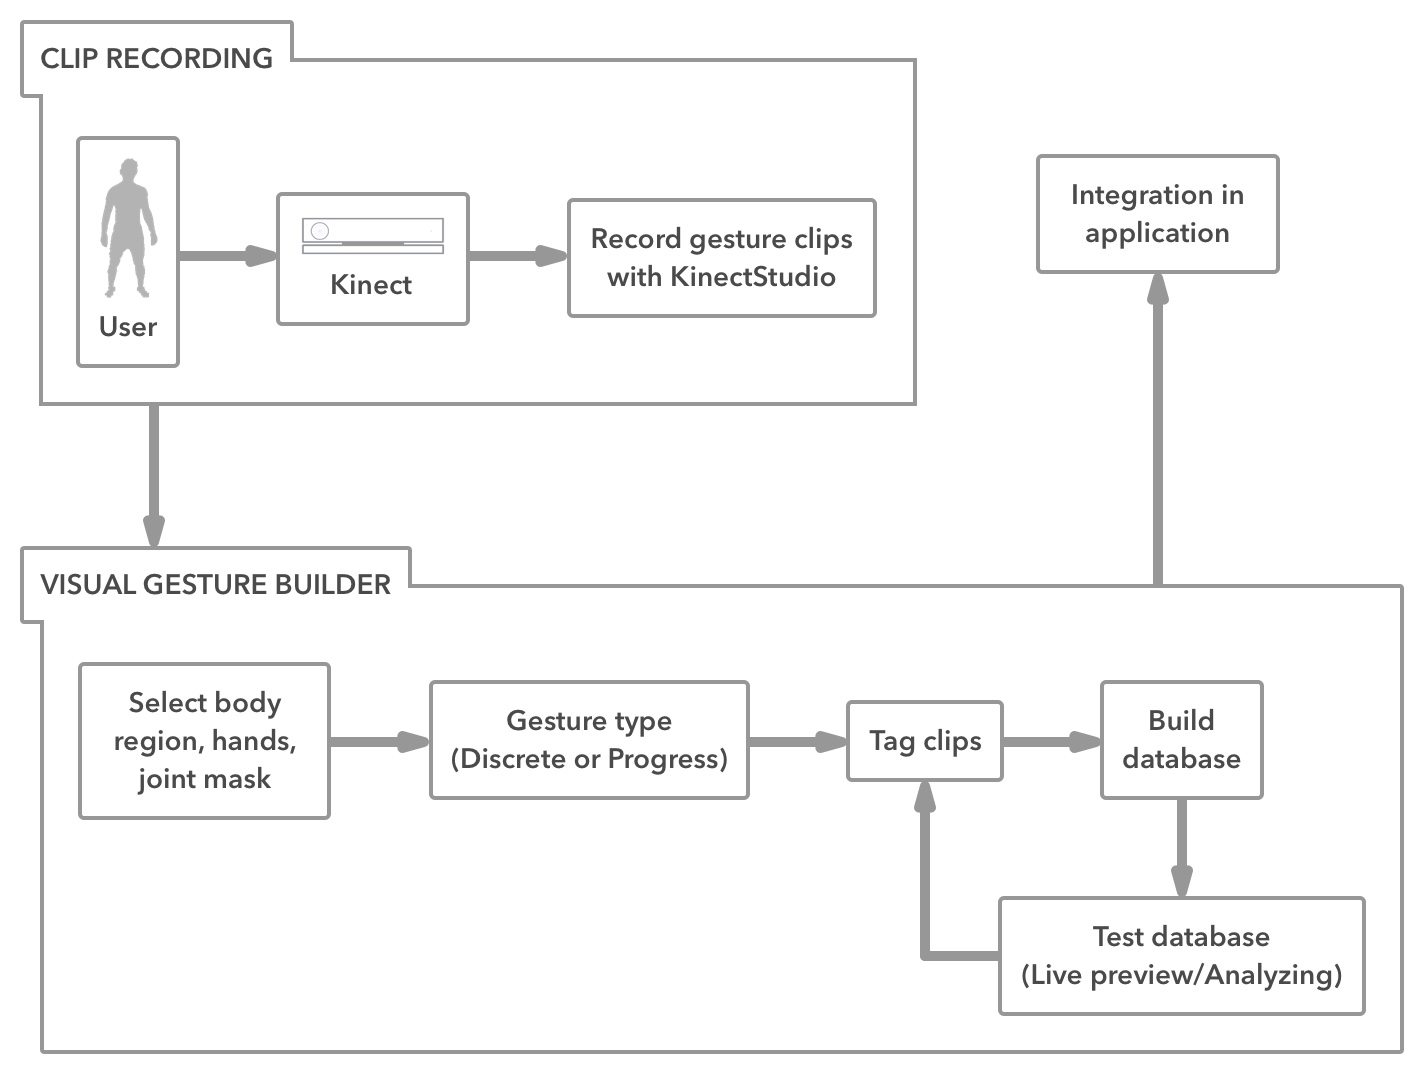
\includegraphics[width=1\linewidth]{Pictures/5_3_gestureCreation}
		\caption{Workflow of creating a gesture database}
		\label{fig:5_3_gestureCreation}
	\end{minipage}
\end{figure}

After the project creation the recordings can be inserted as training data.
The developer has to tag the clips to define a starting as well as an end point of the gesture.
After finishing with tagging a database file can be built.
It is recommended to test it via a live preview or with other recorded clips in a separate analysis area.
If the results are not satisfying, more clips can be recorded and added as training data or existing tags of the clips can be adjusted.
After the testing phase the gesture database file is ready for the integration into the application to detect gestures in runtime. %The structuring of the application architecture is part of the next section.
